% CVPR 2026 camera-ready format
% Machine Learning Assignment 2 -- Kumar Gaurav -- P26AI0006
\documentclass[10pt,twocolumn,letterpaper]{article}

\usepackage{cvpr}
\usepackage{amsmath,amssymb}
\usepackage{booktabs}
\usepackage{graphicx}
\usepackage{xcolor}
\usepackage{url}
\usepackage[breaklinks,colorlinks,allcolors=cvprblue]{hyperref}

\definecolor{cvprblue}{rgb}{0.21,0.49,0.74}

% Tighten float spacing so the eight-page body can hold all required evidence.
\setlength{\textfloatsep}{6pt plus 2pt minus 2pt}
\setlength{\floatsep}{5pt plus 2pt minus 2pt}
\setlength{\intextsep}{5pt plus 2pt minus 2pt}
\setlength{\abovecaptionskip}{3pt}
\setlength{\belowcaptionskip}{0pt}
\renewcommand{\topfraction}{1.0}
\renewcommand{\bottomfraction}{1.0}
\renewcommand{\textfraction}{0.0}
\renewcommand{\floatpagefraction}{1.0}
\renewcommand{\dbltopfraction}{1.0}
\renewcommand{\dblfloatpagefraction}{1.0}

\input{generated/numbers.tex}

\title{When Bagging Beats Boosting:\\
Single Trees, Bootstrap Aggregation, and SAMME\\ on Raw Olivetti Faces}

\author{Kumar Gaurav\\
Roll No. P26AI0006\\
Machine Learning Assignment 2\\
\small Repository: \url{\RepoURL}\\
\small Commit: \texttt{\CommitHash}}

\begin{document}
\maketitle

\begin{abstract}
We study closed-set face identification from raw $64\times64$ Olivetti images
under a frozen, roll-number-seeded split of six training, two validation and two
test images per identity.  We compare a single CART tree, bootstrap aggregation
(bagging) with up to 200 trees, and a from-scratch SAMME multiclass AdaBoost.
Every choice is made on clean validation accuracy; a centred $16\times16$ block
is zeroed only at test time.  The selected single tree overfits (training
accuracy 1.0000, 41 leaves) and reaches 0.6000 validation and 0.5000 test
accuracy.  Bagging with $B=200$ reaches 0.9250 validation and 0.8375 clean test
accuracy, and retains 0.7375 when the central block is zeroed.  SAMME with depth
4 and 50 rounds reaches 0.4375 validation and 0.3875 test accuracy, and 0.2750
masked.  Thirty within-identity bootstrap resamples show that bagging cuts measured
variance by a factor of \BagVarRatio, while squared bias rises from
\TreeFinalBias~to \BagFinalBias; the variance reduction dominates and refit
accuracy improves from \TreeRefitAcc~to \BagRefitAcc.  We report the unsuccessful
and ambiguous outcomes as well: boosting's hard-vote decisions remain weak on
240 training faces, and in a masked case where bagging still gives the true
identity 49 of 200 votes, boosting's normalised score for that identity is only
0.1484.
\end{abstract}

\section{Introduction}

Face identification from raw pixels is a deliberately unfriendly test bed for
classical classifiers.  Each image is a 4096-dimensional vector, only 240
images are available for training, and the forty identities are separated by
subtle lighting, pose and expression changes.  A decision tree can fit this
training set perfectly by isolating individual faces, but such a tree has no
reason to generalise.  Ensembling is the natural response: bagging attacks
variance by averaging trees fitted to bootstrap resamples, while boosting
attacks bias by reweighting examples that the current weak learners get wrong.

This report answers the three assignment questions under one fixed protocol.
The split is generated once from the seed obtained by reading every numeric
character of the roll number \texttt{P26AI0006} in order, namely $\Seed$, and is
reused by every experiment.  It assigns six training, two validation and two
test images to each identity.  Model selection uses clean validation accuracy
only; the clean test set is touched only for final reporting, and the masked
test set is never used for training or selection.  No PCA or other
dimensionality reduction is applied.

Our contributions are: (i) an exact, saved split and a deterministic Q1--Q3
pipeline with artifact checks; (ii) student implementations of bagging and
SAMME, including explicit rejection of random learners; (iii) a diagnostic study
of OOB error, disagreement, margins, weight concentration and masked behaviour;
and (iv) a measured bias--variance decomposition over 30 resamples.  The
headline is that bagging wins clearly, while SAMME is stable but weak: its
weighted training error falls from 0.8500 to 0.6143, yet its test accuracy is
0.3875, below the single tree's 0.5000.

\section{Protocol and Reproducibility}

\subsection{Data and frozen split}

We use \texttt{sklearn.datasets.fetch\_olivetti\_faces}~\cite{samaria1994}: 40
identities, ten images each, $64\times64$ pixels, values in $[0,1]$.  The cache
is stored as \texttt{data/olivetti\_faces.npz}; its image array hashes to
\texttt{\DataHash}.  The seed rule gives
\begin{equation}
\text{seed} = \text{all digits of \texttt{P26AI0006} in order} = \Seed.
\end{equation}
A single \texttt{numpy.random.default\_rng(260006)} stream is consumed identity
by identity in ascending order.  For each identity the ten dataset indices are
permuted once; the first six become training images, the next two validation
images and the last two test images.  The resulting 240/80/80 partition has
SHA-256 \texttt{\SplitHash} and is saved to \texttt{results/split.npz} and
\texttt{results/split.csv}.  Every script loads this file; the split is never
regenerated inside an experiment.

\subsection{Masked test set and selection discipline}

For the masked condition we copy the test matrix and set rows 24--39 and
columns 24--39 of every image to zero, a centred $16\times16$ block.  All other
pixels are unchanged; training and validation images remain clean.  The mask is
applied only when evaluating a fitted model, so this is a response test, not
augmentation.

Every hyperparameter and ensemble size is selected by clean validation
accuracy.  Ties are resolved by the first row in a fixed grid order (shallower
depth, then smaller leaf, then smaller $B$ or fewer rounds).  The clean test and
masked test columns are reported after selection; neither enters a selection
rule.

\subsection{Implementation}

\texttt{scikit-learn}'s~\cite{pedregosa2011}
\texttt{DecisionTreeClassifier} is the only base learner, as permitted.
Bagging and SAMME are implemented in \texttt{src/common.py}.  Bagging draws one
nested sequence of 200 bootstrap replicates and 200 tree seeds; an ensemble of
size $B$ is exactly the first $B$ trees of the 200-tree ensemble, making the
$B$-curve paired rather than a collection of independently seeded runs.  SAMME
fits each tree with the current sample weights, records weighted error,
$\alpha_t$ and the weight distribution, and stops explicitly if a learner is no
better than random.  The full pipeline is \texttt{python -m src.run\_all}; the
run log, resolved configuration, pip freeze and SHA-256 manifests are stored
under \texttt{results/}.  The run took \RuntimeHours~hours.

\section{Q1: Single Trees and Bagging}

\subsection{Decision-tree grid}

The grid crosses maximum depth $\{2,4,8,16,\text{unrestricted}\}$ with minimum
leaf size $\{1,2,4\}$, giving fifteen trees.  Figure~\ref{fig:tree} plots
validation accuracy and the selected leaf size.  Accuracy rises monotonically
with depth; shallow trees underfit badly (depth 2 reaches 0.0750 validation,
depth 16 reaches 0.2875), and the unrestricted tree is the only one above 0.5.
The selected configuration is unrestricted depth with
\texttt{min\_samples\_leaf}$=1$: training 1.0000, validation 0.6000, test
0.5000.  It has \TreeLeaves~leaves, \TreeMeanLeaf~training samples per leaf on
average, and a singleton-leaf fraction of \TreeSingleton.  Perfect training
accuracy on 240 samples is memorisation, not a model of faces.  The complete
grid is in \texttt{results/tree\_grid.csv}.

\begin{figure*}[t]
\centering
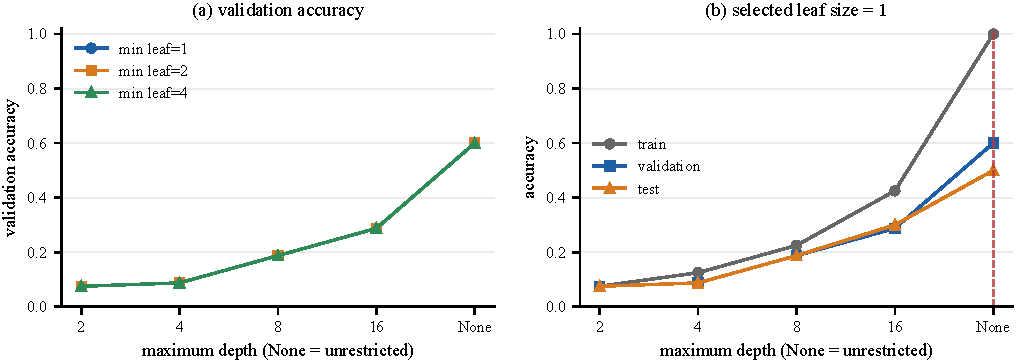
\includegraphics[width=0.86\linewidth]{../figures/fig1_tree_grid.pdf}
\caption{Q1 tree grid.  (a) Validation accuracy for the fifteen depth $\times$
leaf-size combinations; unrestricted depth is the only setting above 0.5.
(b) Train, validation and test accuracy at the selected leaf size 1.  Training
reaches 1.0000 while validation stalls at 0.6000.}
\label{fig:tree}
\end{figure*}

\subsection{Bagging and the ensemble-size curve}

Bagging~\cite{breiman1996,breiman2001} fits $B$ trees to bootstrap resamples of
the 240 training images and predicts by plurality vote.
Table~\ref{tab:bagging} and Figure~\ref{fig:bagging} report
$B\in\{1,5,10,25,50,100,200\}$.  A single bootstrap tree ($B=1$) reaches 0.4625
validation and 0.3875 test accuracy, worse than the tree fitted to all training
data.  Averaging fixes this quickly: $B=10$ gives 0.7625 validation, $B=50$
gives 0.8500, and $B=200$ gives 0.9250 validation and 0.8375 test accuracy.
Training accuracy is already 1.0000 at $B=10$; further trees reduce variance,
not training error.  $B=200$ is selected for its highest validation accuracy;
$B=100$ is close (0.9000 validation) and reaches the same 0.8375 test accuracy.

\input{generated/tables/bagging.tex}

\begin{figure*}[t]
\centering
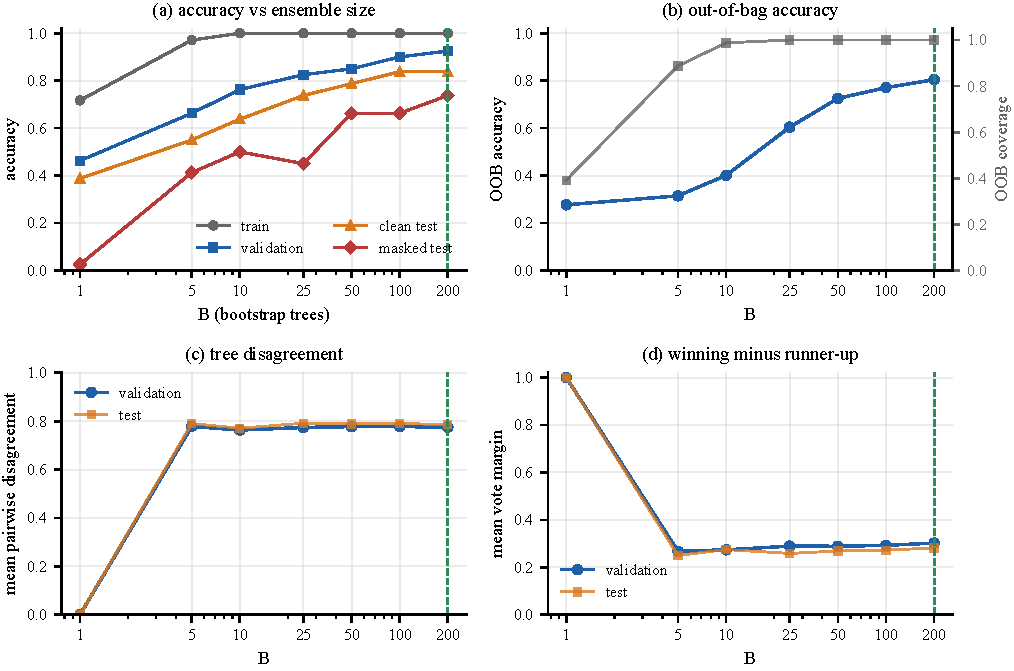
\includegraphics[width=0.86\linewidth]{../figures/fig2_bagging.pdf}
\caption{Bagging diagnostics: (a) accuracy versus $B$; (b) out-of-bag accuracy
and coverage; (c) mean pairwise tree disagreement; (d) mean winning-minus-runner-up
vote margin.  The dashed line marks the selected $B=200$.}
\label{fig:bagging}
\end{figure*}

\subsection{Out-of-bag error, disagreement and margin}

Out-of-bag accuracy at $B=200$ is \BagOOB, close to the 0.8375 test estimate and
well above the single tree's 0.5000.  Coverage is 1.0: every training image is
out of bag for at least one tree.  The mean number of distinct training indices
per bootstrap sample is \BagDistinct, against the theoretical
\BagDistinctTheory, confirming with-replacement sampling.

Trees disagree on \BagDis~of validation pairs on average.  This is healthy
diversity: if every tree made the same error, averaging could not help.  The
mean winning-minus-runner-up vote margin is \BagMargin, so the winner holds
about 30 percentage points more votes than the runner-up.  The relationship is
not monotone in $B$ (0.2675 at $B=5$ to 0.3023 at $B=200$) because adding trees
can move both the winner and the runner-up.  OOB accuracy and margin improve
with $B$, while disagreement jumps to about 0.78 by $B=5$ and then stays almost
flat.  Disagreement measures diversity, not correctness; OOB accuracy and
margin track accuracy.

\subsection{Clean versus masked test, and face cases}

The masked column of Table~\ref{tab:bagging} is the most striking Q1 result.  A
single bootstrap tree falls to 0.0250 masked accuracy: it has learned splits on
the central pixels and has no redundancy when they are removed.  Five trees
already recover 0.4125; 200 trees reach 0.7375, only 0.1000 below their clean
accuracy.  Averaging makes the prediction robust to destroying one local region
even though individual trees are not region-invariant.

Confidence reinforces the difference.  On clean images the selected tree's mean
winning confidence is \TreeCleanConf~and bagging's is \BagCleanConf; under the
mask they are \TreeMaskConf~and \BagMaskConf.  The tree is maximally confident
in both conditions, including when wrong, while bagging's confidence falls with
its accuracy.  Vote fractions are not calibrated probabilities, but they are
sensitive to lost evidence.

Figure~\ref{fig:q1cases} shows two faces where bagging corrects the tree and two
where both fail.  For dataset index 376 (true 37) the tree predicts 3 with
probability 1.0; bagging gives 37 \CaseOneVotes~of 200 votes, a margin of
\CaseOneMargin.  For index 175 (true 17) the tree predicts 22; bagging gives 17
\CaseTwoVotes~votes, margin \CaseTwoMargin.  Among shared errors, index 2
(true 0) is predicted 26 by the tree and 15 by bagging
(\CaseThreeVotes~votes, margin \CaseThreeMargin), while index 154 (true 15) is
predicted 5 by both (\CaseFourVotes~votes, margin \CaseFourMargin).  Bagging
corrects 28 of the 40 test faces the tree gets wrong; on the other 12 both fail.
These shared errors are confident, visually plausible confusions, not
tie-breaking noise.  Bagging fixes variance-driven errors on unstable splits,
but not systematic confusions shared by all bootstrap trees.

\begin{figure*}[t]
\centering
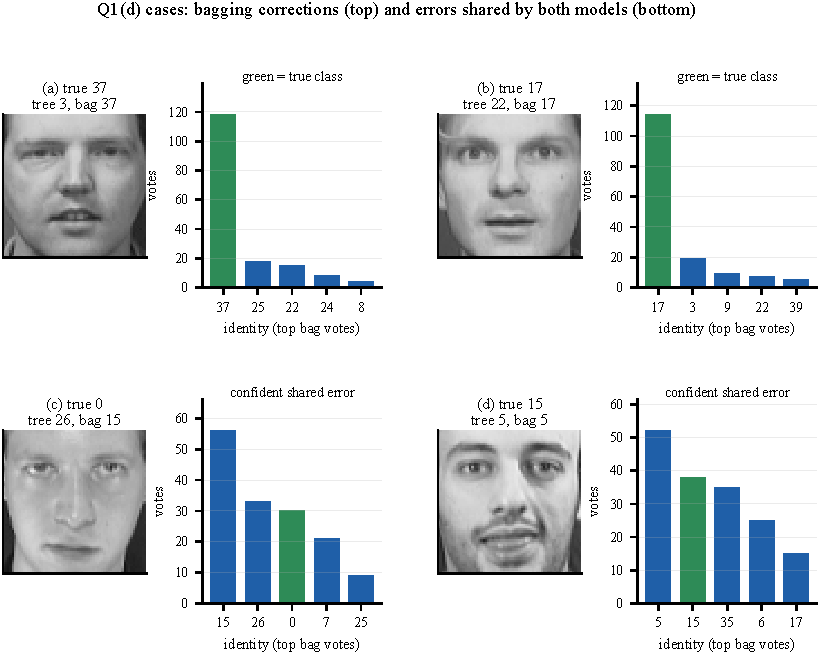
\includegraphics[width=0.86\linewidth]{../figures/fig3_q1_cases.pdf}
\caption{Q1 case studies.  Top: faces where bagging corrects the single tree
(indices 376 and 175).  Bottom: faces where both fail (indices 2 and 154).  Bars
show the five largest bag vote counts; the true identity is green when present.}
\label{fig:q1cases}
\end{figure*}

\section{Q2: SAMME Boosting}

\subsection{Algorithm and numerical safeguards}

SAMME~\cite{zhu2009,freund1997} is multiclass AdaBoost with hard-label weak
learners.  With $K=40$ classes and training weights $w_i^{(1)}=1/n$, round $t$
fits a tree $h_t$ on the weighted training set, computes
\begin{equation}
\epsilon_t=\sum_{i=1}^{n} w_i^{(t)}\mathbf{1}[h_t(x_i)\neq y_i],
\end{equation}
and, if $\epsilon_t<1-1/K$, assigns
\begin{equation}
\alpha_t=\log\frac{1-\epsilon_t}{\epsilon_t}+\log(K-1).
\label{eq:alpha}
\end{equation}
Weights are updated by
\begin{equation}
w_i^{(t+1)}=\frac{w_i^{(t)}\exp\!\left(\alpha_t\mathbf{1}[h_t(x_i)\neq y_i]\right)}
{\sum_{j=1}^{n}w_j^{(t)}\exp\!\left(\alpha_t\mathbf{1}[h_t(x_j)\neq y_j]\right)}.
\label{eq:update}
\end{equation}
The ensemble score is $S_k(x)=\sum_{t=1}^{T}\alpha_t\mathbf{1}[h_t(x)=k]$, and
the normalised response is
\begin{equation}
q_k(x)=\frac{S_k(x)}{\sum_{t=1}^{T}\alpha_t},\qquad \sum_{k=1}^{K}q_k(x)=1.
\label{eq:q}
\end{equation}
The prediction is $\arg\max_k q_k(x)$.

Two edge cases are explicit.  If $\epsilon_t\ge 1-1/K$, the learner is no better
than random and $\alpha_t\le 0$; we reject the round, record the reason in
\texttt{stop\_reason}, and stop rather than assign a meaningless weight.  If
$\epsilon_t\le\varepsilon$ with $\varepsilon=10^{-12}$, we clip the error so
$\alpha_t$ stays finite.  In this run no round was rejected: every requested
round produced $\epsilon_t<0.975$.

\subsection{One complete toy round}

Table~\ref{tab:toy} works through a three-class, nine-sample, one-dimensional
problem with three samples per class and a depth-1 stump.  The stump predicts
class 1 for the three class-2 samples, so $\epsilon_1=3/9=1/3$ and
$\alpha_1=\log(2)+\log(2)=1.3863$.  The six correct samples are multiplied by
$e^0=1$ and the three wrong samples by $e^{\alpha_1}=4$; after normalisation the
correct weights are $1/18=0.0556$ and the wrong weights are $2/9=0.2222$.  The
updated weights sum to 1.0000, exactly the behaviour required by
Eqs.~\eqref{eq:alpha}--\eqref{eq:update}: hard samples receive four times the
weight of easy samples before normalisation.

\input{generated/tables/toy.tex}

\subsection{Depth $\times$ rounds grid}

Table~\ref{tab:boostgrid} summarises the 16-run grid (depths 1--4, requested
rounds 10, 25, 50 and 100).  All 16 runs accepted every requested round.  Depth
1 is too weak: at 100 rounds validation accuracy is only 0.1000.  Depth 4 is
clearly better, peaking at 50 rounds with 0.4375 validation and 0.3875 test
accuracy.  More rounds are not monotonically better: 100 rounds at depth 4
gives 0.4250 validation, slightly below 50 rounds, while training accuracy is
0.9708 at 50 rounds and the last weighted error is 0.6143.  The selected model
is therefore depth 4, 50 rounds, not the largest grid cell.  Its last
$\alpha_t$ is \BoostAlphaLast, and the 100-round run's final weighted error
(0.6694) is higher than the 50-round run's, so additional rounds fit hard faces
rather than improving the ensemble.

\input{generated/tables/boosting_grid.tex}

\subsection{Twenty-five, fifty and one hundred learners}

Table~\ref{tab:boostvsbag} compares bagging and boosting at the three requested
ensemble sizes with frozen settings.  Bagging wins at every size: 0.7375,
0.7875 and 0.8375 test accuracy at 25, 50 and 100 trees, versus 0.2875, 0.3875
and 0.3750 for SAMME.  Bagging also trains faster in serial-equivalent time at
25 and 50 learners; at 100 the gap narrows because each boosting round refits a
depth-4 tree on reweighted data.  The comparison is controlled: both families
see the same 240 training images, validation set and test set, and the bagging
column uses the same nested bootstrap sequence as Table~\ref{tab:bagging}.  Its
times are sums of per-tree fit times, not wall-clock times distorted by parallel
scheduling.

\input{generated/tables/boost_vs_bag.tex}

\subsection{The face that receives the largest weight}

Figure~\ref{fig:weight} follows dataset index 79 (identity 7), the training face
with the largest final SAMME weight.  Its final weight is \WeightFinal, against
a uniform weight of \WeightUniform---about twenty-one times larger.  It is
misclassified by \WeightNMiss~of the \WeightRounds~weak learners, yet the
cumulative ensemble predicts it correctly from round \WeightFirstCorrect.  This
is the point of boosting: the face is hard for individual depth-4 trees, so its
weight grows, but accumulated votes are already correct and become more so as
later learners specialise.  Figure~\ref{fig:weight}(b) shows the mechanism: a
correct round reduces the weight sharply, but the next tree usually errs again,
so the weight climbs back.  The top ten training faces hold 0.4481 of the total
weight, so reweighting is concentrated.

\begin{figure*}[t]
\centering
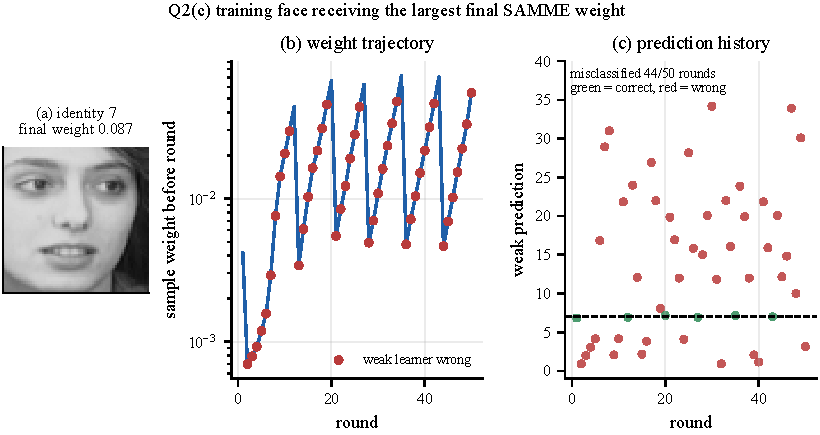
\includegraphics[width=0.82\linewidth]{../figures/fig5_weight_case.pdf}
\caption{Training face with the largest final SAMME weight (dataset index 79,
identity 7).  (a) Face and final weight.  (b) Weight before each round on a log
scale; red points mark rounds where the weak learner is wrong.  (c) Weak-learner
prediction by round, with the true identity dashed.}
\label{fig:weight}
\end{figure*}

\subsection{Masked response}

Figure~\ref{fig:mask} studies dataset index 170 (true identity 17), a test face
that all three clean models classify correctly.  Full clean and masked
accuracies and mean winning confidences are in Table~\ref{tab:final}; here we
focus on the face where the ensembles diverge.  After masking, the single tree
predicts 13, bagging predicts 17 with \MaskBagTrueVotes~of 200 votes and margin
\MaskBagMargin, and boosting predicts 3.  Boosting's normalised score for the
true identity is only \MaskBoostTrueQ, while its score for identity 3 is 0.1807;
the top-two margin is \MaskBoostMargin.  Bagging's tree disagreement rises from
0.7613 clean to \MaskBagDis~masked, so the ensemble is genuinely uncertain, but
the true class still leads by 49 votes.  The mask removes 256 central pixels,
where many identity-specific contours live.  Bagging survives because its trees
make different errors; boosting's weighted vote is dominated by learners that
overfitted to the clean central region.  Its reweighted training distribution
concentrates on a few hard faces (top ten: 0.4481; heaviest: 0.0872), so later
learners specialise on clean central features and have no fallback when that
region is removed, whereas bagging still has 49 trees on the true identity.

\begin{figure*}[t]
\centering
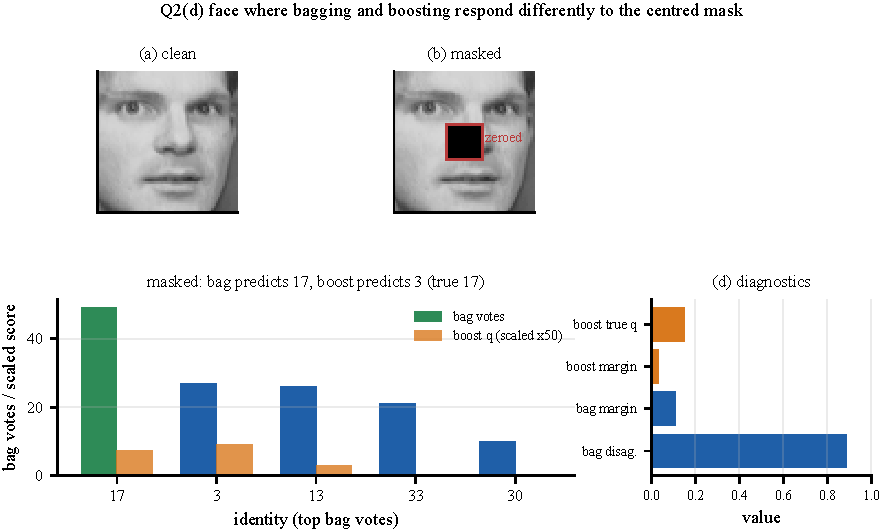
\includegraphics[width=0.82\linewidth]{../figures/fig6_mask_case.pdf}
\caption{Masked-response case (dataset index 170, true identity 17).  (a) Clean
image.  (b) Image with the centred $16\times16$ block zeroed.  (c) Bag votes and
scaled boosting scores for the top five identities.  (d) Disagreement and
margin diagnostics.  Bagging predicts 17; boosting predicts 3.}
\label{fig:mask}
\end{figure*}

\section{Q3: Measured Bias and Variance}

\subsection{Estimator and resampling design}

For a fixed test image $x_i$ with one-hot target $e_i$, let $p_r(x_i)$ be the
probability vector from refit $r$ and
$\bar p(x_i)=\frac{1}{R}\sum_{r=1}^{R}p_r(x_i)$.  We measure
\begin{equation}
\mathrm{Bias}^2=\frac{1}{N}\sum_{i=1}^{N}\lVert \bar p(x_i)-e_i\rVert_2^2,
\end{equation}
\begin{equation}
\mathrm{Var}=\frac{1}{NR}\sum_{i=1}^{N}\sum_{r=1}^{R}
\lVert p_r(x_i)-\bar p(x_i)\rVert_2^2.
\label{eq:var}
\end{equation}
This is the assignment's Euclidean probability decomposition~\cite{hastie2009},
not the zero-one loss decomposition~\cite{kohavi1996,domingos2000}; the two need
not agree, and accuracy is reported separately.

We draw $R=30$ within-identity bootstrap training sets.  For each identity we
sample six of its six training images with replacement, so every resample has
240 images and the same 6/2/2 identity structure as the original split.  The
selected tree, the 200-tree bag and SAMME (depth 4, 50 rounds) are refitted from
scratch and evaluated on the same 80 clean test images.  Resample indices are
saved in \texttt{results/q3\_resamples.npz}; per-refit probabilities are in
\texttt{results/q3\_predictions.npz}.

\subsection{Selected models}

Table~\ref{tab:final} and Figure~\ref{fig:biasvar}(a) give the measured
decomposition.  The single tree has bias$^2$ \TreeFinalBias~and variance
\TreeFinalVar.  Bagging has bias$^2$ \BagFinalBias~and variance \BagFinalVar:
variance falls by a factor of \BagVarRatio, while squared bias rises by
\BagBiasDelta.  The variance reduction dominates, so accuracy improves.  This
is the expected trade-off: averaging vote fractions shrinks spread across
resamples but also pulls the mean prediction away from a one-hot target.
Boosting has bias$^2$ \BoostFinalBias~and variance \BoostFinalVar.  Its variance
is also low, but its bias is \BoostBiasRatio~times the tree's, consistent with
its low accuracy: depth-4 weak learners are stable but not expressive enough,
and hard-vote SAMME does not recover the missing signal.  Averaged over 30
refits, the tree's accuracy is \TreeRefitAcc~$\pm$~\TreeRefitStd, bagging's is
\BagRefitAcc~$\pm$~\BagRefitStd, and boosting's is
\BoostRefitAcc~$\pm$~\BoostRefitStd.  The ranking matches the single split,
though bagging's refit mean (\BagRefitAcc) is below its single-split estimate
(\BagCleanAcc).

\input{generated/tables/final.tex}

\begin{figure*}[t]
\centering
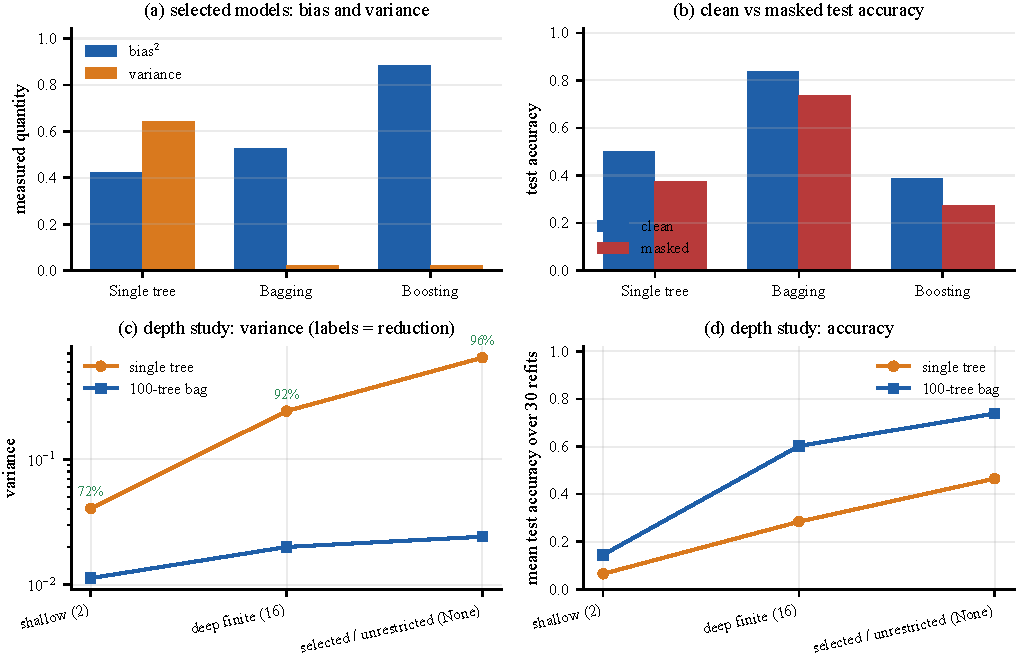
\includegraphics[width=0.86\linewidth]{../figures/fig7_bias_variance.pdf}
\caption{Q3 results.  (a) Measured squared bias and variance for the selected
models over 30 within-identity resamples.  (b) Clean and masked test accuracy.
(c) Variance of the single tree and a 100-tree bag at three depths, with
percentage reduction printed above each pair.  (d) Mean test accuracy over the
same 30 refits.}
\label{fig:biasvar}
\end{figure*}

\subsection{Depth study}

The selected tree is unrestricted, so ``deeper than selected'' is not defined.
We compare a shallow tree (depth 2), a deep finite tree (depth 16) and the
selected unrestricted tree (depth \texttt{None}), each with a matched 100-tree
bag.  Figure~\ref{fig:biasvar}(c,d) gives the results.

Depth 2 has only \DepthShallowLeaves~leaves (mean occupancy
\DepthShallowMeanLeaf, singleton fraction \DepthShallowSingleton); it underfits,
with bias$^2$ \DepthShallowSingleBias, variance \DepthShallowSingleVar~and
accuracy \DepthShallowSingleAcc.  Its bag raises accuracy to
\DepthShallowBagAcc, but bias stays at \DepthShallowBagBias.  Depth 16 has
\DepthMidLeaves~leaves and variance \DepthMidSingleVar; the bag cuts variance by
\DepthMidVarRed\% and raises accuracy from \DepthMidSingleAcc~to
\DepthMidBagAcc.  The unrestricted tree has \DepthDeepLeaves~leaves (mean
occupancy \DepthDeepMeanLeaf), variance \DepthDeepSingleVar~and disagreement
\DepthDeepDis; its bag cuts variance by \DepthDeepVarRed\%, but raises bias from
\DepthDeepSingleBias~to \DepthDeepBagBias, and raises accuracy to
\DepthDeepBagAcc.

The largest accuracy gain is at depth \LargestImprovementDepth
(\LargestImprovementGain).  Thus the answer to the assignment's question is
\textbf{\DeepestLargest}: the deepest tree is not necessarily the depth at which
bagging gives the largest accuracy improvement.  The deepest tree is where
bagging removes the most variance---\DepthDeepVarRed\% versus \DepthMidVarRed\%
at depth 16 and \DepthShallowVarRed\% at depth 2---because it has the most leaves
and the largest across-resample variance.  But the extra variance removal is
partly offset by a larger bias increase: bagging raises bias from
\DepthDeepSingleBias~to \DepthDeepBagBias~at unrestricted depth, compared with
\DepthMidSingleBias~to \DepthMidBagBias~at depth 16.

Disagreement rules out a simple ``more diversity is better'' explanation.
Pairwise disagreement between the 100 bagged trees is highest for shallow trees
(\DepthShallowDis), lower at depth 16 (\DepthMidDis) and lowest at unrestricted
depth (\DepthDeepDis).  Deep trees converge on the same clean-training
partition, so they disagree less with each other, even though their predictions
move most when the training set is resampled.  Disagreement measures diversity
within one ensemble; variance measures sensitivity across resamples.  Leaf
occupancy explains the other half: depth 2 cannot fit the identities, while the
unrestricted tree is most extreme.  Depth 16 has enough leaves but a smaller
bias penalty from bagging, which is why its accuracy gain is largest.  Variance
reduction is necessary for the gain, but not sufficient when bias also grows.

Table~\ref{tab:final} answers the stability question directly.  Boosting has
the lowest variance in probability space (\BoostVar, marginally below bagging's
\BagVar), but its refit accuracy is \BoostRefitAcc~$\pm$~\BoostRefitStd, so low
variance does not imply good predictions: its bias dominates.  Bagging has the
smallest accuracy standard deviation (\BagRefitStd) and the best clean and
masked accuracy.  The single tree has the largest clean-to-masked drop
(\TreeCleanDrop, versus \BagCleanDrop~for bagging and \BoostCleanDrop~for
boosting), and is maximally confident in both conditions.

\section{Discussion}

Bagging wins because the unrestricted tree has relatively low bias and high
variance~\cite{dietterich2000}: it represents the training set almost perfectly,
but a different bootstrap sample produces different axis-aligned splits.
Averaging 200 such trees removes almost all variance (a factor of \BagVarRatio)
at the cost of a modest bias increase (\BagBiasDelta), which is why bagging gains
0.3375 test accuracy over the single tree and loses only 0.1000 under the mask.

SAMME is designed for weak learners slightly better than random.  With 40
classes the random threshold is 0.975, and a depth-4 tree on 240 faces has
weighted error around 0.61, so it is accepted but weak.  Reweighting then
concentrates on a small set of hard faces (top ten: 0.4481), reducing effective
sample size and making the next tree more specialised.  The result is stable but
biased: variance is low, bias is high, and 100 rounds do not beat 50.  Soft
probabilities, more data, or stronger weak learners would likely help, but lie
outside the frozen protocol.

The mask is a best-case test for ensemble diversity and a worst-case test for
models relying on the central face.  A single bootstrap tree collapses to 0.0250
masked accuracy, the selected tree drops from 0.5000 to 0.3750, bagging from
0.8375 to 0.7375, and boosting from 0.3875 to 0.2750; the ordering is unchanged,
but bagging retains a vote lead while boosting's score flips identity.

\paragraph{Limitations.}  The test set has only 80 images, so one image is 1.25
accuracy points.  All results come from one split and one seed, as required; the
30 resamples estimate refit variability but are not cross-validation.  The
bias--variance numbers use the Euclidean probability decomposition and are not
directly comparable to zero-one decompositions.

\section{Conclusion}

Under a frozen, roll-number-seeded 6/2/2 split and raw 4096-pixel inputs,
bagging is the clear winner: 200 bootstrap trees reach 0.9250 validation and
0.8375 clean test accuracy, and 0.7375 with a centred $16\times16$ test block
zeroed.  A single unrestricted tree overfits and reaches 0.5000.  A from-scratch
SAMME implementation is correct and stable---its toy round matches the
closed-form weights, and weighted error falls from 0.8500 to 0.6143---but its
hard-vote decisions remain weak at 0.3875.  The measured decomposition explains
the ranking: bagging cuts variance relative to a matched tree, especially at
unrestricted depth, while boosting's low variance is offset by high bias.

{
\small
\bibliographystyle{ieeenat_fullname}
\bibliography{main}
}

\end{document}
